\section{Experimental results}
\label{sec:experiments}

\subsection{Arithmetic datasets}
\label{sec:arithmetic-dataset}

The arithmetic dataset is a replica of the "simple function task" in \citet{trask-nalu}.
The goal is to sum two random contiguous subsets of a vector and apply an arithmetic operation as defined in \eqref{eq:arithmetic-problem}
\begin{equation}
t = \sum_{i = s_{1,\mathrm{start}}}^{s_{1,\mathrm{end}}} x_i \circ \sum_{i = s_{2,\mathrm{start}}}^{s_{2,\mathrm{end}}} x_i \quad \text{where } \mathbf{x} \in \mathbb{R}^n, x_i \sim \mathrm{Uniform}[r_{\mathrm{lower}}, r_{\mathrm{upper}}], \circ \in \{+, -, \times\}
\label{eq:arithmetic-problem}
\end{equation}
where $n$ (default $100$), $U[r_{\mathrm{lower}}, r_{\mathrm{upper}}]$ (interpolation default is $U[1,2]$ and extrapolation default is $U[2,6]$), and other dataset parameters are used to assess learning capability (see details in appendix \ref{sec:appendix:simple-function-task:data-generation} and the effect of varying the parameters in appendix \ref{sec:appendix-simple-function-task:dataset-parameter-effect}).

\subsubsection{Model evaluation}
We define the success-criterion as a solution that is acceptably close to a perfect solution.
To evaluate if a model instance solves the task consistently we compare the MSE to a nearly-perfect solution on the extrapolation range over multiple seeds.
If $\mathbf{W}_1, \mathbf{W}_2$ defines the weights of the fitted model, $\mathbf{W}_1^\epsilon$ is nearly-perfect and $\mathbf{W}_2^*$ is perfect (example in equation \ref{eq:nearly-perfect-solution-example}), then the criteria for successful convergence is $\mathcal{L}_{\mathbf{W}_1, \mathbf{W}_2} < \mathcal{L}_{\mathbf{W}_1^\epsilon, \mathbf{W}_2^*}$, measured on the extrapolation error, for $\epsilon = 10^{-5}$. We report a 95\% confidence interval using a binomial distribution \cite{wilson-binomial}.
\begin{equation}
    \mathbf{W}_1^\epsilon = \begin{bmatrix}
    1 - \epsilon & 1 - \epsilon & 0 + \epsilon & 0 + \epsilon \\
    1 - \epsilon & 1 - \epsilon & 1 - \epsilon & 1 - \epsilon
    \end{bmatrix}, \mathbf{W}_2^* = \begin{bmatrix}
    1 & 1
    \end{bmatrix}
    \label{eq:nearly-perfect-solution-example}
\end{equation}
To measure speed of convergence of the first iteration for which $\mathcal{L}_{\mathbf{W}_1, \mathbf{W}_2} < \mathcal{L}_{\mathbf{W}_1^\epsilon, \mathbf{W}_2^*}$ is reported with a 95\% confidence interval, calculated using a gamma distribution with maximum likelihood profiling. Only models that solved the task are included.

We assume an approximate discrete solution with parameters close to $\{-1, 0, 1\}$ is important for inferring exact arithmetic operations.
To measure the sparsity we introduce a sparsity error (defined in equation \ref{eq:sparsity-error}).
Similar to the convergence metric we only include model instances that did solve the task and report the 95\% confidence interval, which is calculated using a beta distribution with maximum likelihood profiling.
\begin{equation}
E_\mathrm{sparsity} = \max_{h_{\ell-1}, h_{\ell}} \min(|W_{h_{\ell-1},h_\ell}|, |1 - |W_{h_{\ell-1},h_\ell}||)
\label{eq:sparsity-error}
\end{equation}

We choose the optimal set of parameters based on the validation dataset (interpolation range).

\subsubsection{Arithmetic operation comparison}
We compare models on different arithmetic operation $\circ \in \{+, -, \times\}$. The multiplication models, NMU and $\mathrm{NAC}_{\bullet}$, have an addition layer first, either NAU or $\mathrm{NAC}_{+}$, followed by a multiplication layer. The addition models are just two layers of the same unit. The NALU model consists of two NALU layers. See explicit definitions and regularization values in appendix \ref{sec:appendix:comparison-all-models}.

Each experiment is trained for $5 \cdot 10^6$ iterations (details in appendix \ref{sec:appendix:comparison-all-models}). Results are presented in table \ref{tab:function-task-static-defaults}. For multiplication, the NMU succeeds more often and converge faster. For addition NAU is comparable to a linear transformation in success-rate and convergence speed, but is more sparse. However, for subtraction a linear transformation can not consistently solve the task, while NAU and $\mathrm{NAC}_{+}$ solves it. A larger comparison is in appendix \ref{sec:appendix:comparison-all-models} and an ablation study is in appendix \ref{sec:appendix:ablation-study}.

\begin{table}[!h]

\caption{\label{tab:function-task-static-defaults}Shows the success-rate for $\mathcal{L}_{\mathbf{W}_1, \mathbf{W}_2} < \mathcal{L}_{\mathbf{W}_1^\epsilon, \mathbf{W}_2^*}$, at what global step the model converged at, and the sparsity error for all weight matrices.}
\centering
\begin{tabular}{crllll}
\toprule
\multicolumn{1}{c}{Op} & \multicolumn{1}{c}{Model} & \multicolumn{1}{c}{Success} & \multicolumn{2}{c}{Solved at} & \multicolumn{1}{c}{Sparsity error} \\
\cmidrule(l{3pt}r{3pt}){1-1} \cmidrule(l{3pt}r{3pt}){2-2} \cmidrule(l{3pt}r{3pt}){3-3} \cmidrule(l{3pt}r{3pt}){4-5} \cmidrule(l{3pt}r{3pt}){6-6}
 &  & Rate & Median & Mean & Mean\\
\midrule
 & $\mathrm{NAC}_{\bullet}$ & $30\%$ & $2.5 \cdot 10^{6}$ & $2.5 \cdot 10^{6} \pm 1.5 \cdot 10^{6}$ & $\mathbf{3.9 \cdot 10^{-4} \pm 9.4 \cdot 10^{-4}}$\\

 & Linear & $0\%$ & --- & --- & ---\\

 & NALU & $0\%$ & --- & --- & ---\\

\multirow{-4}{*}{\centering\arraybackslash $\bm{\times}$} & NMU & $\mathbf{90\%}$ & $\mathbf{1.4 \cdot 10^{6}}$ & $\mathbf{1.6 \cdot 10^{6} \pm 5.6 \cdot 10^{5}}$ & $1.8 \cdot 10^{-3} \pm 1.1 \cdot 10^{-3}$\\
\cmidrule{1-6}
 & $\mathrm{NAC}_{+}$ & $\mathbf{100\%}$ & $6.0 \cdot 10^{4}$ & $7.1 \cdot 10^{4} \pm 2.4 \cdot 10^{4}$ & $4.8 \cdot 10^{-1} \pm 2.0 \cdot 10^{-2}$\\

 & Linear & $\mathbf{100\%}$ & $4.2 \cdot 10^{4}$ & $\mathbf{4.2 \cdot 10^{4} \pm 1.9 \cdot 10^{3}}$ & $6.1 \cdot 10^{-1} \pm 1.2 \cdot 10^{-1}$\\

 & NALU & $0\%$ & --- & --- & ---\\

\multirow{-4}{*}{\centering\arraybackslash $\bm{+}$} & NAU & $\mathbf{100\%}$ & $\mathbf{1.8 \cdot 10^{4}}$ & $7.0 \cdot 10^{5} \pm 9.2 \cdot 10^{5}$ & $\mathbf{1.7 \cdot 10^{-3} \pm 8.0 \cdot 10^{-4}}$\\
\cmidrule{1-6}
 & $\mathrm{NAC}_{+}$ & $\mathbf{100\%}$ & $8.0 \cdot 10^{3}$ & $1.5 \cdot 10^{6} \pm 1.5 \cdot 10^{6}$ & $4.6 \cdot 10^{-1} \pm 2.9 \cdot 10^{-2}$\\

 & Linear & $\mathbf{100\%}$ & $1.1 \cdot 10^{6}$ & $1.9 \cdot 10^{6} \pm 1.3 \cdot 10^{6}$ & $3.7 \cdot 10^{-1} \pm 1.1 \cdot 10^{-1}$\\

 & NALU & $20\%$ & $3.6 \cdot 10^{6}$ & $3.6 \cdot 10^{6} \pm 1.3 \cdot 10^{7}$ & $4.7 \cdot 10^{-1} \pm 3.3 \cdot 10^{-1}$\\

\multirow{-4}{*}{\centering\arraybackslash $\bm{-}$} & NAU & $\mathbf{100\%}$ & $\mathbf{4.0 \cdot 10^{3}}$ & $\mathbf{4.2 \cdot 10^{3} \pm 3.0 \cdot 10^{2}}$ & $\mathbf{1.9 \cdot 10^{-3} \pm 4.2 \cdot 10^{-4}}$\\
\bottomrule
\end{tabular}
\end{table}


\subsubsection{Evaluating theoretical claims}

To validate our theoretical claim, that the NMU model works better than $\mathrm{NAC}_{\bullet}$ for larger $H_{\ell-1}$, we increase the hidden size of the network, thereby adding redundant units. Redundant units are very common neural networks, where fitting an unknown function is often done by overparameterization.

Additionally, the NMU model is unlike the $NAC_{\bullet}$ model also capable of handling inputs that are both negative and positive. To validate this empirically, the training and validation datasets are sampled for $\mathrm{U}[-2,2]$, and then tested on $\mathrm{U}[-6,-2] \cup \mathrm{U}[2,6]$. The other ranges are defined in Appendix \ref{sec:appendix-simple-function-task:dataset-parameter-effect}.

Finally, for a fair comparison we introduce two new units: A variant of $\mathrm{NAC}_{\bullet}$ called $\mathrm{NAC}_{\bullet, \sigma}$, that only supports multiplication, by constraining the weights with $W = \sigma(\hat{W})$. And a variant, called $\mathrm{NAC}_{\bullet, \mathrm{NMU}}$, that uses linear weights and sparsity regularization, identically to that of the NMU.

Figure \ref{fig:simple-function-static-theoreical-claims-experiment} shows that the NMU can both handle a much larger hidden-size, negative inputs, and that solving the division and bias issues alone improves the success rate, but are not sufficient when the hidden-size is large, as there is no ideal initialization. Interestingly, none of the models can learn the $\mathrm{U}[-1.1,1.2]$, suggesting that certain input distributions might be troublesome to learn.

\begin{figure}[h]
\centering
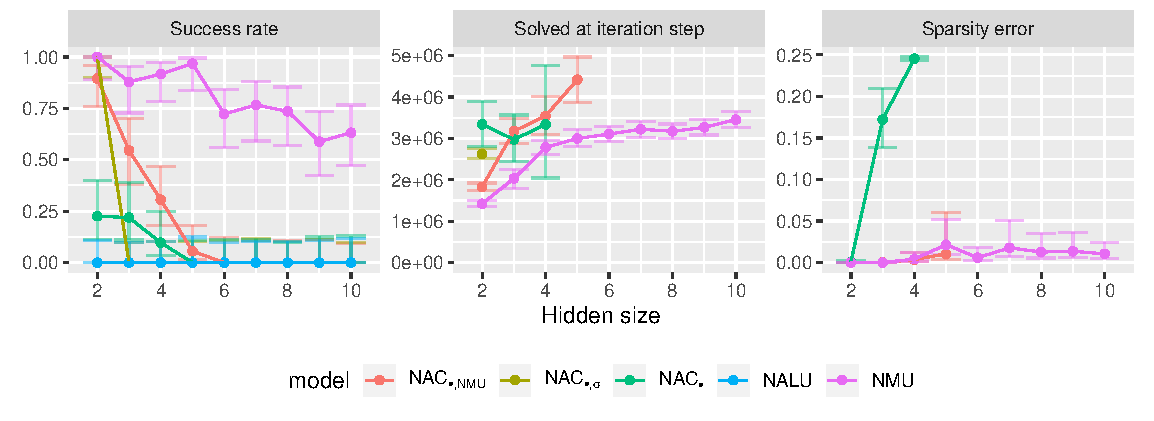
\includegraphics[width=\linewidth,trim={0 1.3cm 0 0},clip]{results/simple_function_static_mul_hidden_size_short.pdf}
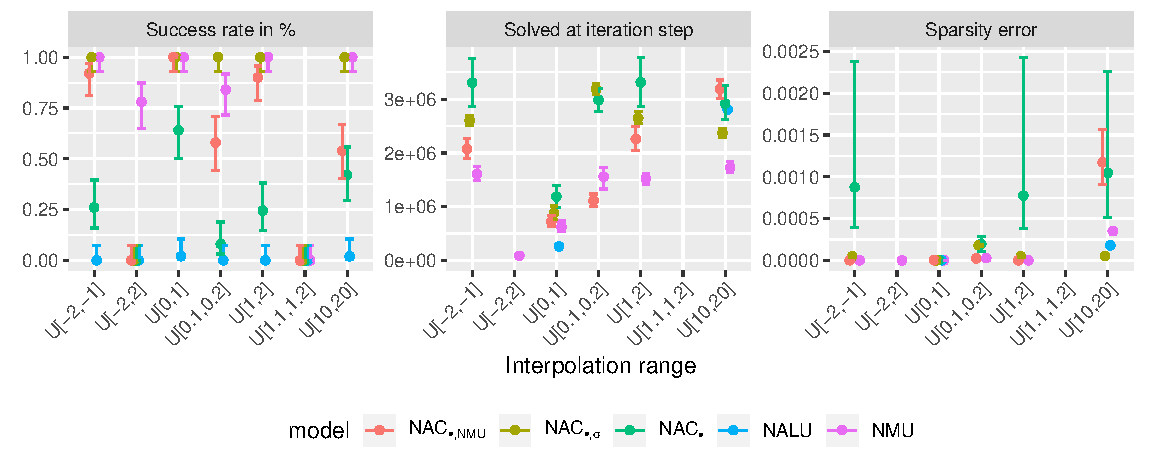
\includegraphics[width=\linewidth,trim={0 0.5cm 0 0.775cm},clip]{results/simple_function_static_mul_range.pdf}
\caption{Shows that the NMU can handle a large hidden size, and works when the input contains both positive and negative numbers ($U[-2,2]$),  extrapolation ranges are defined in Appendix \ref{sec:appendix-simple-function-task:dataset-parameter-effect}.} 
%\caption{Shows the effect of the dataset parameters. For each interpolation range, the following extrapolation ranges are used: ${\mathrm{U}[-2,2] \rightarrow \mathrm{U}[-6,-2] \cup \mathrm{U}[2,6]}$, ${\mathrm{U}[0,1] \rightarrow \mathrm{U}[1,5]}$, ${\mathrm{U}[0.1,0.2] \rightarrow \mathrm{U}[0.2,2]}$, ${\mathrm{U}[1,2] \rightarrow \mathrm{U}[2,6]}$, ${\mathrm{U}[10, 20] \rightarrow \mathrm{U}[20, 40]}$. The uniform sampling ranges are chosen to test the effect of mean, variance, and sign for optimizing.}
\label{fig:simple-function-static-theoreical-claims-experiment}
\end{figure}

\subsection{Product of sequential MNIST}

To investigate if a deep neural network can be learned when backpropagating through an arithmetic layer, the arithmetic layers are used as a recurrent-unit to a sequence of MNIST digits, where the target is to fit the cumulative product. This task is similar to ``MNIST Counting and Arithmetic Tasks'' in \citet{trask-nalu}\footnote{The same CNN is used, \url{https://github.com/pytorch/examples/tree/master/mnist}.}, but uses multiplication rather than addition. Each model is trained on sequences of length 2, and then tested on sequences of length up to 20 MNIST digits.

We define the success-criterion by comparing the MSE of each model with a baseline model that has a correct solution for the arithmetic layer. If the MSE of each model, is less than the upper 1\% MSE-confidence-interval of the baseline model, then the model is considered successfully converged.

Sparsity and ``solved at iteration step'' is determined as described in experiment \ref{sec:arithmetic-dataset}. The validation set is the last 5000 MNIST digits from the training set, which is used to select the best epoch.

In this experiment we found that having an unconstrained ``input-network'' can cause the multiplication-units to learn an undesired solution, e.g. $(0.1 \cdot 81 + 1 - 0.1) = 9$. This solves the problem with a similar success-rate, but not in the intended way. To prevent such solution, we regularize the CNN output with $\mathcal{R}_{\mathrm{z}} = \frac{1}{H_{\ell-1} H_\ell} \sum_{h_\ell}^{H_\ell} \sum_{h_{\ell-1}}^{H_{\ell-1}} (1 - W_{h_{\ell-1},h_\ell}) \cdot (1 - \bar{z}_{h_{\ell-1}})^2$. This regularizer is applied to the NMU and $\mathrm{NAC}_{\bullet,\mathrm{NMU}}$ models. See appendix \ref{sec:appendix:sequential-mnist:ablation} for the results, when this regularizer is not used.

Figure \ref{fig:sequential-mnist-prod-results} shows that the NMU does not hinder learning a more complex neural network. And that it can extrapolate to much longer sequences than what it is trained on.

\begin{figure}[h]
\centering
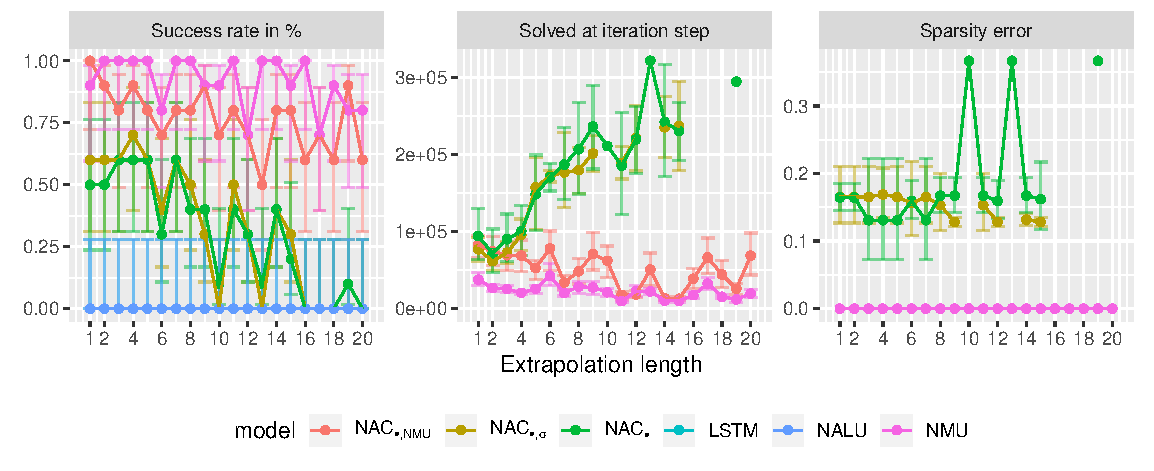
\includegraphics[width=\linewidth,trim={0 0.5cm 0 0},clip]{results/sequential_mnist_prod_long.pdf}
\caption{Shows the ability of each model to backpropagate and extrapolate to longer sequences.} 
\label{fig:sequential-mnist-prod-results}
\end{figure}
